\documentclass[a4paper,10pt,ngerman]{scrartcl}
\usepackage{babel}
\usepackage[T1]{fontenc}
\usepackage[utf8x]{inputenc}
\usepackage[a4paper,margin=2.5cm,footskip=0.5cm]{geometry}
\usepackage{graphicx}
\newcommand{\Aufgabe}{Aufgabe 1: Schmucknachrichten}
\newcommand{\TeilnahmeId}{76626}                 
\newcommand{\Name}{Quirin Klemm}            


% Kopf- und Fußzeilen
\usepackage{scrlayer-scrpage, lastpage}
\setkomafont{pageheadfoot}{\large\textrm}
\lohead{\Aufgabe}
\rohead{Teilnahme-ID: \TeilnahmeId}
\cfoot*{\thepage{}/\pageref{LastPage}}

% Position des Titels
\usepackage{titling}
\setlength{\droptitle}{-1.0cm}

% Für mathematische Befehle und Symbole
\usepackage{amsmath}
\usepackage{amssymb}

% Für Bilder
\usepackage{graphicx}

% Für Algorithmen
\usepackage{algpseudocode}

% Für Quelltext
\usepackage{listings}
\usepackage{color}
\definecolor{mygreen}{rgb}{0,0.6,0}
\definecolor{mygray}{rgb}{0.5,0.5,0.5}
\definecolor{mymauve}{rgb}{0.58,0,0.82}
\lstset{
  keywordstyle=\color{blue},commentstyle=\color{mygreen},
  stringstyle=\color{mymauve},rulecolor=\color{black},
  basicstyle=\footnotesize\ttfamily,numberstyle=\tiny\color{mygray},
  captionpos=b, % sets the caption-position to bottom
  keepspaces=true, % keeps spaces in text
  numbers=left, numbersep=5pt, showspaces=false,showstringspaces=true,
  showtabs=false, stepnumber=2, tabsize=2, title=\lstname
}
\lstdefinelanguage{JavaScript}{ % JavaScript ist als einzige Sprache noch nicht vordefiniert
  keywords={break, case, catch, continue, debugger, default, delete, do, else, finally, for, function, if, in, instanceof, new, return, switch, this, throw, try, typeof, var, void, while, with},
  morecomment=[l]{//},
  morecomment=[s]{/*}{*/},
  morestring=[b]',
  morestring=[b]",
  sensitive=true
}

% Diese beiden Pakete müssen zuletzt geladen werden
%\usepackage{hyperref} % Anklickbare Links im Dokument
\usepackage{cleveref}

% Daten für die Titelseite
\title{\textbf{\Huge\Aufgabe}}
\author{\LARGE Teilnahme-ID: \LARGE \TeilnahmeId \\\\
	    \LARGE Bearbeiter/-in dieser Aufgabe: \\ 
	    \LARGE \Name\\\\}
\date{\LARGE\today}

\begin{document}

\maketitle
\tableofcontents

\vspace{0.5cm}

\clearpage
\section{Lösungsidee}
Eine Nachricht besteht aus mehreren unterschiedlichen Buchstaben. 
Für jeden Buchstaben ist ein Codewort zu finden, wobei insgesamt ein präfixfreier Code entstehen muss.
Dabei soll die Gesamtlänge der codierten Nachricht möglichst gering sein.
Daher wird ein präfixfreier Code gesucht, bei dem häufig vorkommende Buchstaben kurze Codewörter erhalten, während seltenere Buchstaben längere Codewörter zugewiesen bekommen. 
Im Allgemeinen gilt, solange alle Perlen im Durchmesser gleich sind:
\begin{equation}
  \label{Kosten eines Buchstaben}
  c_i = p_i \cdot n_i
\end{equation}

\begin{equation}
  \label{equation:simple_kostenberechnung}
  l = \sum_i c_i
\end{equation}

wobei:\\
- $c_i$ die Kosten des Buchstaben $i$ ist,\\
- \( p_i \) die Häufigkeit des Buchstabens \( i \) in der Nachricht darstellt,  \\
- \( n_i \) die Länge des Codewortes für den Buchstaben \( i \) ist,  \\
- \( l \) die Länge der codierten Nachricht ist. \\ 
Wenn sich die Durchmesser der Perlen unterscheiden, stimmt diese Gleichung nicht mehr und muss anders berechnet werden.\\
\\
Um präfixfreien Code zu erzeugen, wird am besten ein Baum benutzt. Da man durch diesen sicher gehen kann, das keine Codewort der Präfix eines anderen Codewort ist. 
Dabei ist jedes Blatt des Baums ein Codewort und jede Kante zu dem Blatt eine Code vom Codewort. Der Baum hat mindestens so viele Blätter wie es verschiedene Buchstaben gibt.
Jeder innerne Knoten hat dabei maximal so viele Kinder, wie es verschiedene Perlen gibt. Die Ebene des Blattes entspricht die Länge des Codewortes.

\begin{figure}[h]
  \centering
  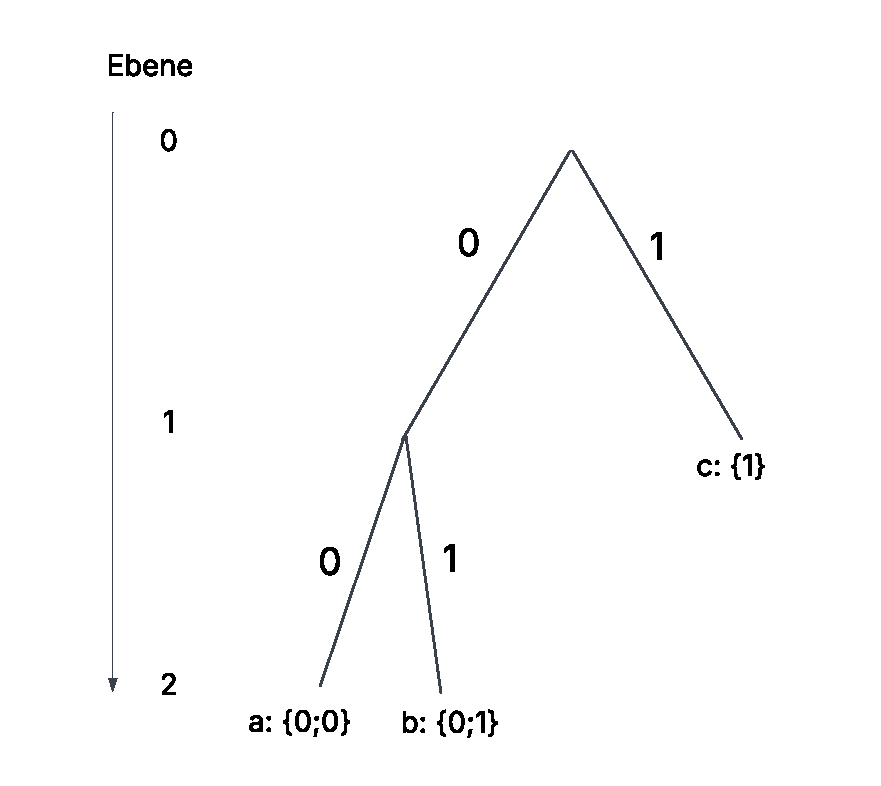
\includegraphics[width=0.6\textwidth]{Schmucknachrichten/pdf_src/simple_tree.pdf}
  \caption{simple tree}
  \label{fig:simple tree}
\end{figure}

\subsection{Perlen besitzen gleichen Durchmesser}
Um möglichst kleinen präfixfreien Code zu erstellen, muss der Buchstaben der am öftesten vorkommt ganz oben eingeordnet werden und die nächsten Buchstaben dann in absteigender Reihenfolge. 
In Abbildung \ref{fig:simple tree} hätte c die höchste Häufigkeit und dannach kommt a und b. Was von a und b die höhere Häufigkeit hat, ist egal, da sie beide auf der untersten Ebene sind.\\
Daher ergibt sich $p_1 \geq p_2 \geq p_3 ... \geq p_i$ und $n_1 \leq n_2 \leq n_3 ... \leq n_i$\\
Zu finden ist also ein Baum, der basierden auf den Häufigkeiten der Buchstaben, seine Blätter so auf seine Ebene so verteilt, dass die Gleichung \eqref{equation:simple_kostenberechnung} möglichst gering ist. 
Jeder innerne Knoten muss dabei mindestens zwei Kinder haben, da ein innerner Knoten mit nur einem Kind die Äste des Baums verlängert ohne irgendwelche anderen Vorteile dem Baum zu bringen.\\

Zu Beginn des Algorithmus wird ein perfekt ausbalancierter Baum erstellt, der so viele Blätter wie Buchstaben hat (Abbildung \ref{fig:balancierter_Baum}). 
Jedes Blatt wird von links nach rechts in aufsteigender Reihenfolge mit einem Buchstaben belegt, und die Gesamtkosten des Baums werden gemäß der Formel (1) berechnet. 
Dabei ergeben sich deutlich höhere Kosten für die rechten Blätter des Baums im Vergleich zu den linken, da alle Blätter auf derselben Ebene sind, jedoch die Häufigkeit der Buchstaben auf der rechten Seite größer ist.
Um das auszugleichen, wird das Blatt mit den höchsten Kosten eine Ebene nach oben verschoben. 
Dies geschieht indem der Elternknoten des Blattes selber zum Blatt wird und alle Kinder verliert.
Dadurch hat der Baum insgesammt zu wenig Blätter, weshalb er erweitert werden muss.
Dies geschieht indem, alle möglichen neuen Blätter angeschaut werden und das mit den geringsten Kosten hinzugefügt wird. (Abbildung \ref{fig:trans_1})\\
Das nach oben verschobenene Blatt erhält den Zusatz $protected$. Das verhindert, dass es sselbst weitere Kinder bekommen kann.
Dadurch wird ein Zyklus vermieden, bei dem ein Blatt zunächst nach oben verschoben und anschließend wieder nach unten erweitert würde.
Das nach oben Verschieben und unten Neueinfügen der Blätter gilt als ein Optimierungsschritt,
welcher im Optimierungsprozess wiederholt wird. (Abbildung \ref{fig:trans_2})
Dieser Vorgang wird so lange fortgesetzt, bis keine Blätter mehr verschoben werden können (Abbildung \ref{fig:baum_fertig}) - also keine weitern Optimierungen mehr möglich sind.
Am Ende wird der Baum mit den geringsten Gesamtkosten ausgegeben.


\vspace{3em}


\begin{figure}[h]
  \centering
  \begin{minipage}{0.49\textwidth}
    \centering
    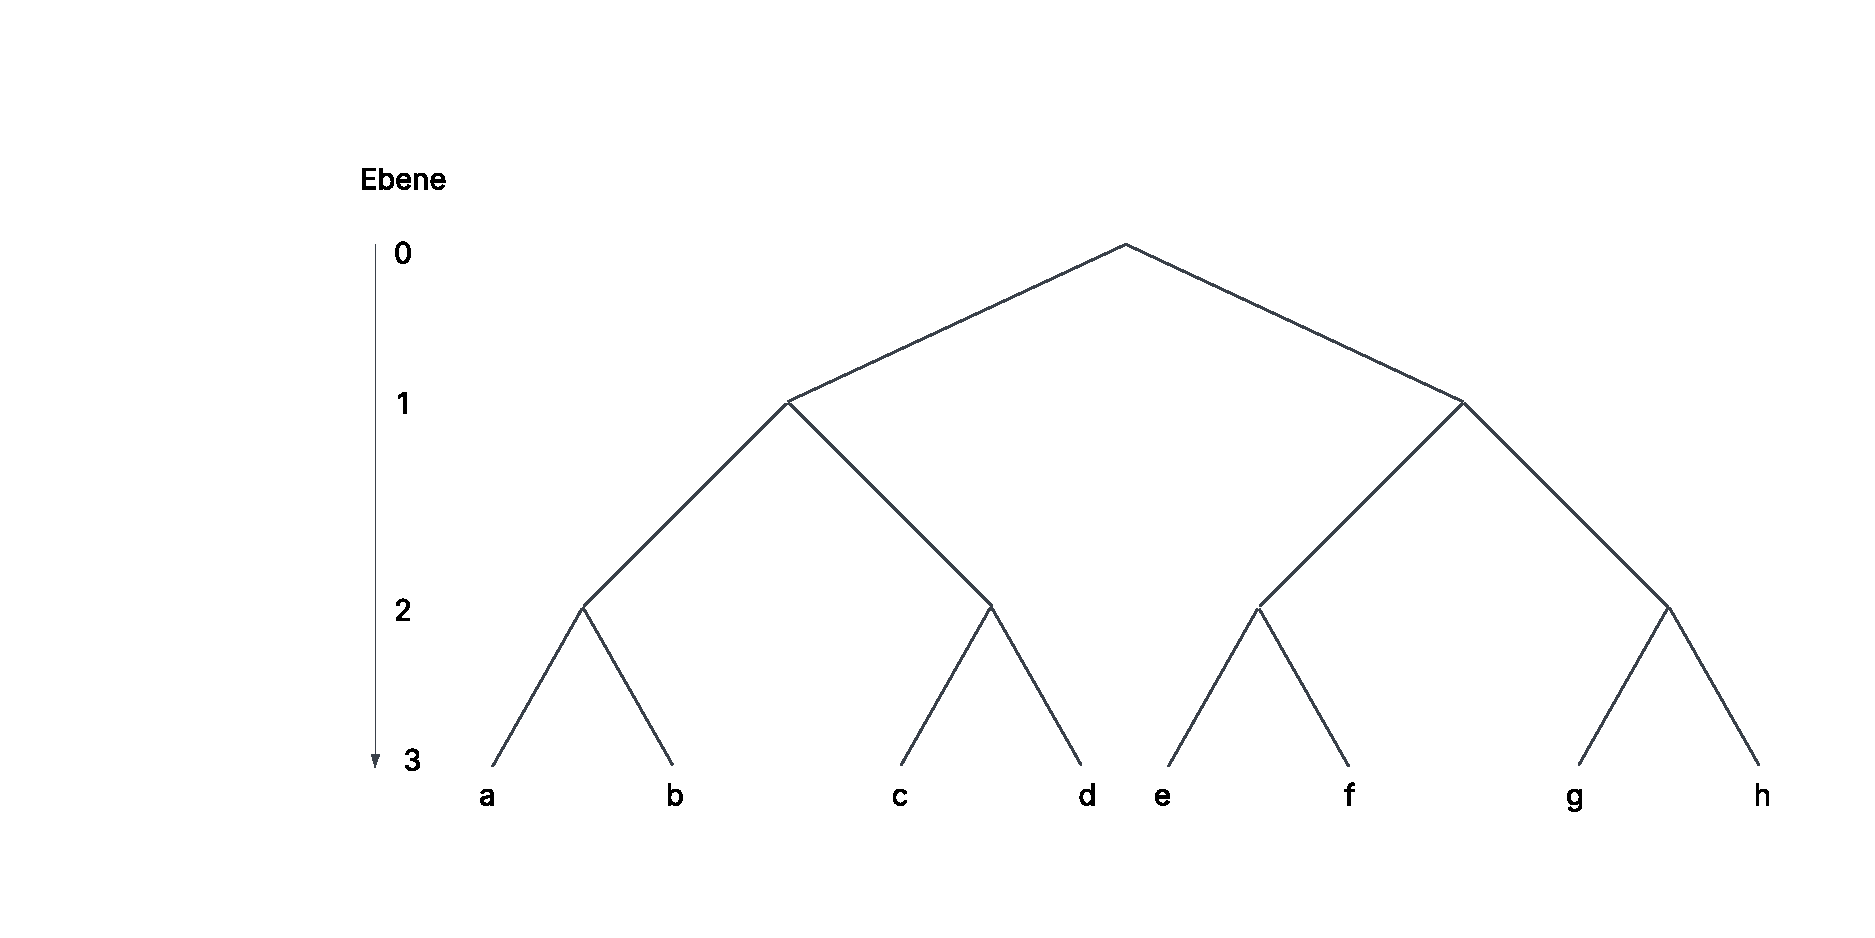
\includegraphics[width=\textwidth]{Schmucknachrichten/pdf_src/trans_1.pdf}
    \caption{Balancierter Baum}
    \label{fig:balancierter_Baum}
  \end{minipage}
  \hfill
  \begin{minipage}{0.49\textwidth}
    \centering
    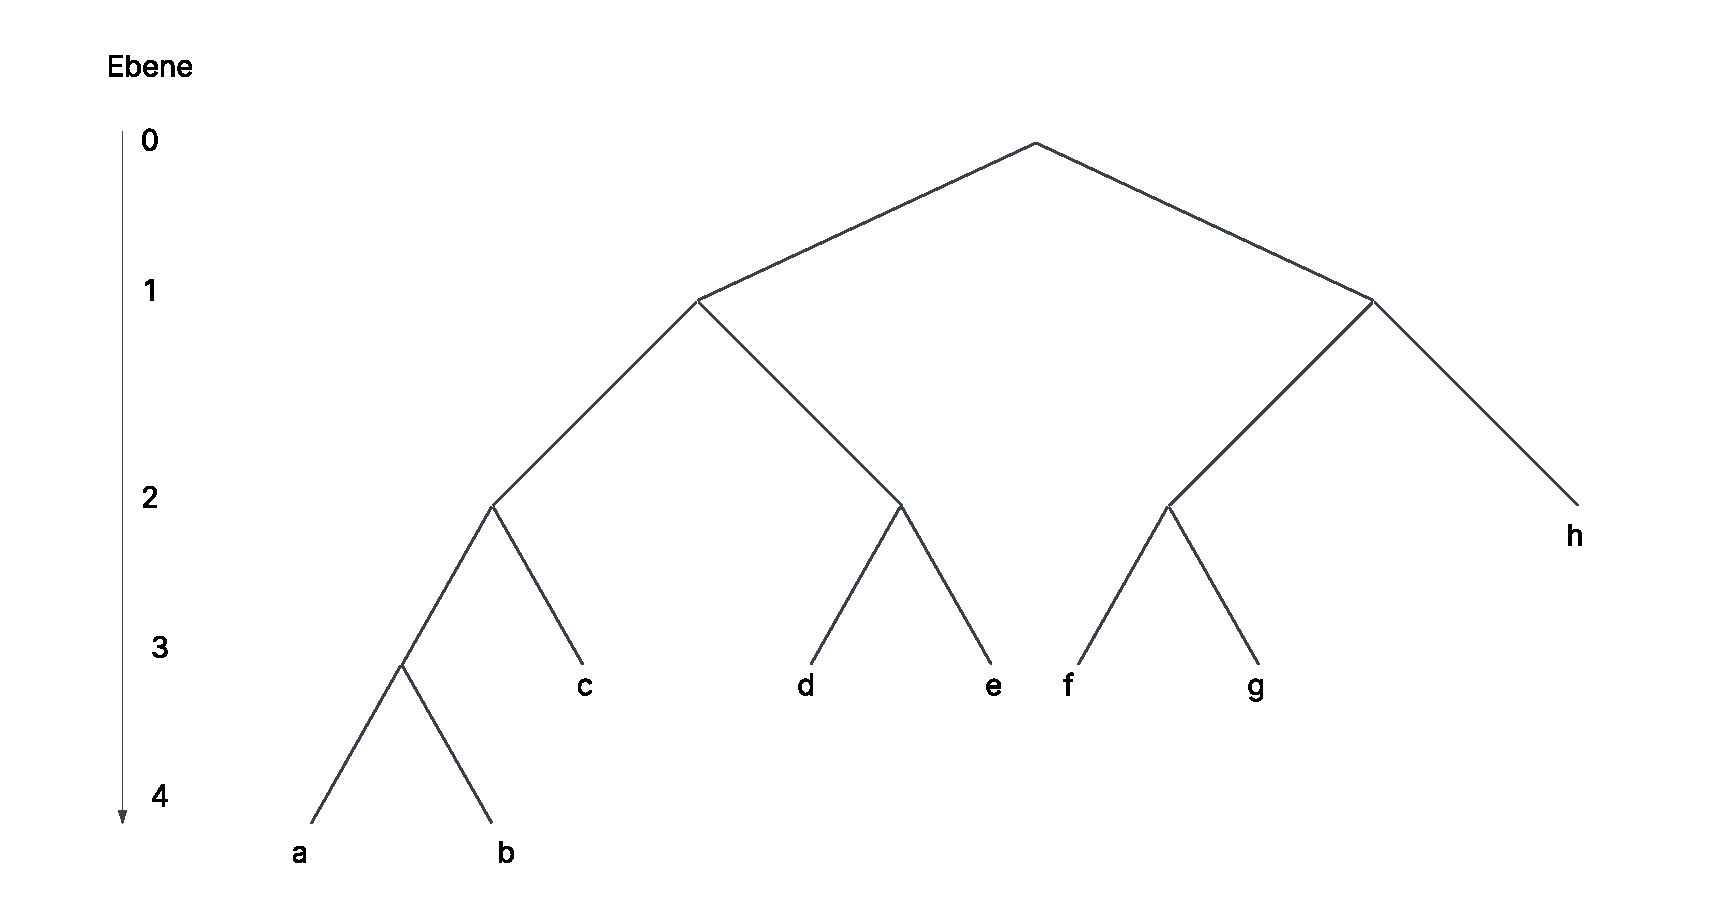
\includegraphics[width=\textwidth]{Schmucknachrichten/pdf_src/trans_2.pdf}
    \caption{Transformation 1}
    \label{fig:trans_1}
  \end{minipage}
\end{figure}

\begin{figure}[h]
  \centering
  \begin{minipage}{0.49\textwidth}
    \centering
    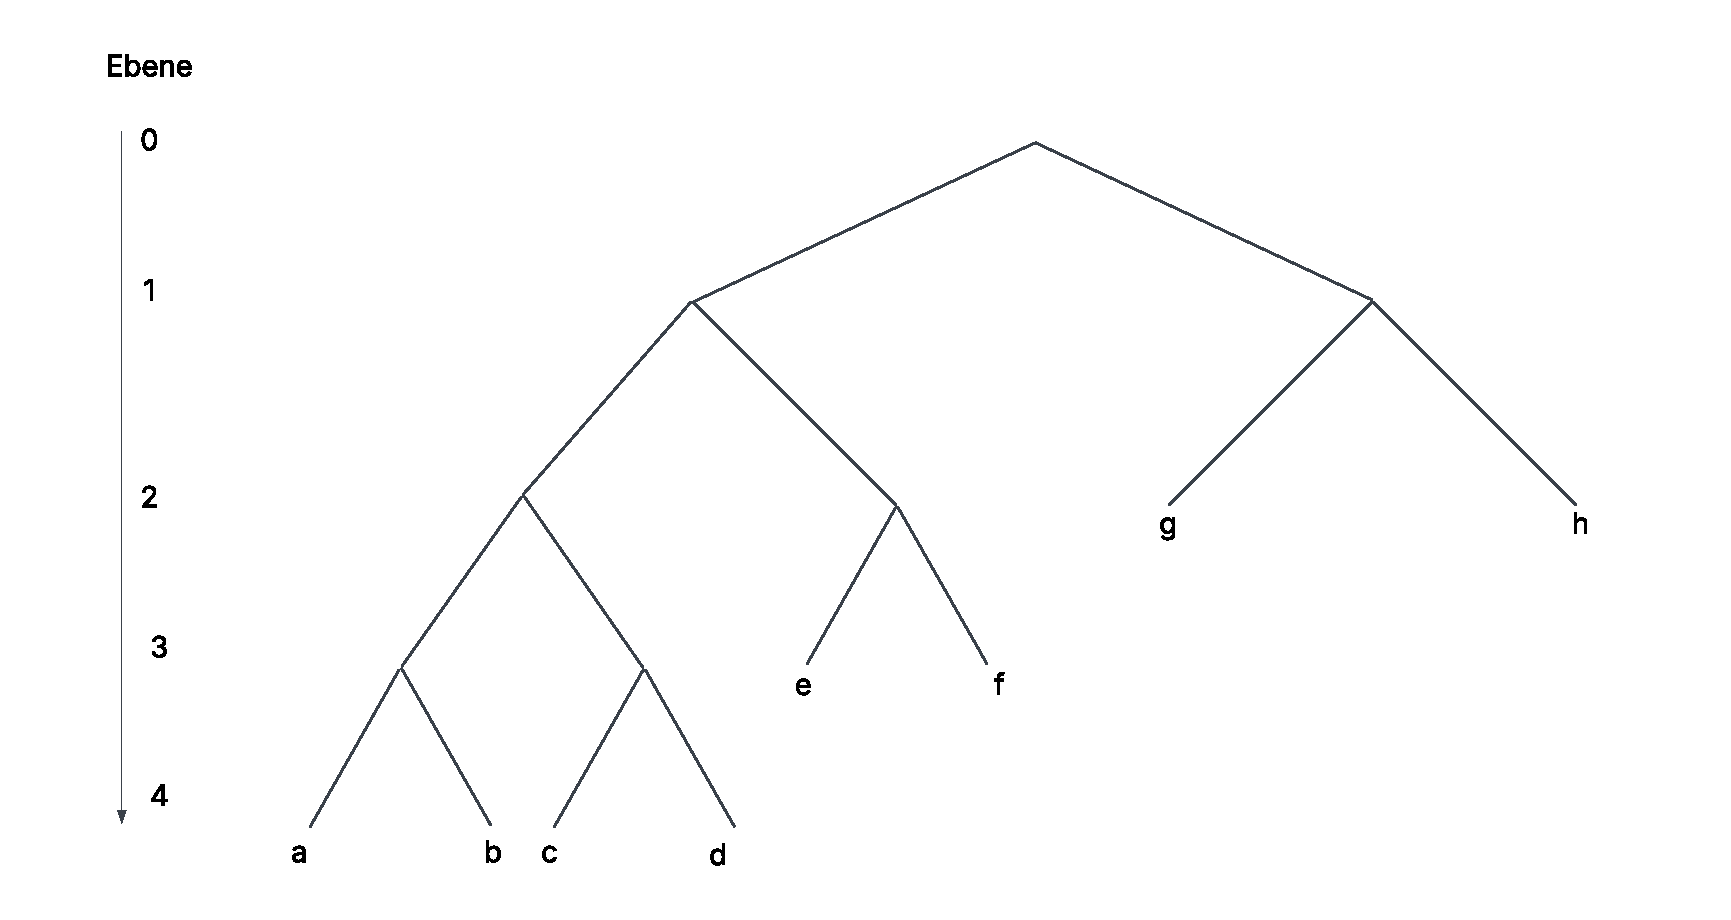
\includegraphics[width=\textwidth]{Schmucknachrichten/pdf_src/trans_3.pdf}
    \caption{Transformation 2}
    \label{fig:trans_2}
  \end{minipage}
  \hfill
  \begin{minipage}{0.3\textwidth}
    \centering
    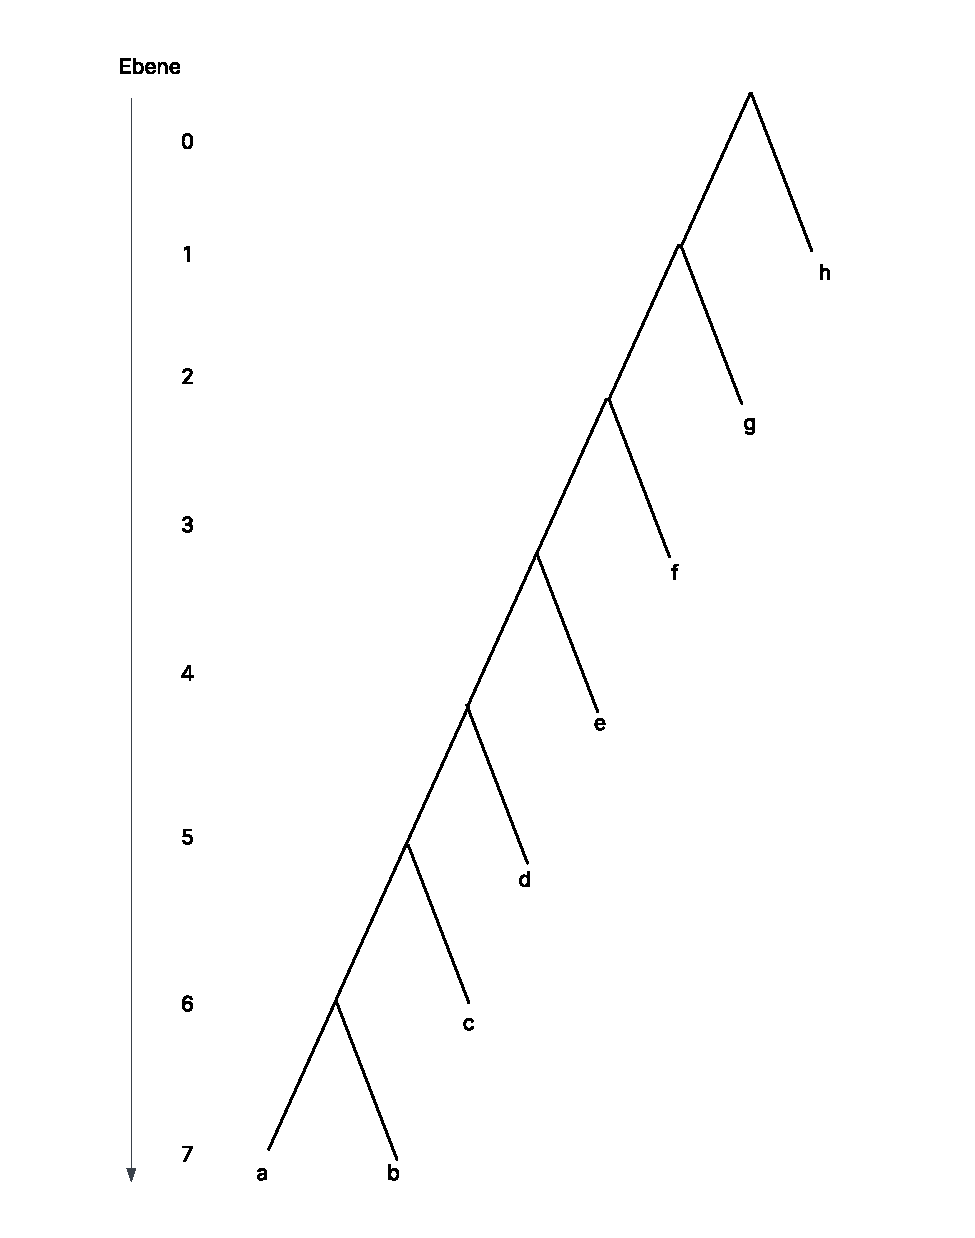
\includegraphics[width=\textwidth]{Schmucknachrichten/pdf_src/trans_4.pdf}
    \caption{Ausgearteter Baum}
    \label{fig:baum_fertig}
  \end{minipage}
\end{figure}

\clearpage
\subsection{Perlen mit unterschiedlichen Durchmesser}
Das Problem bei unterschiedlichen Durchmesser besteht darin, dass Blätter auf derselben Ebene unterschiedliche Kosten haben können.
Daher stimmt die Gleichung \eqref{Kosten eines Buchstaben} nicht mehr, und muss statt dessen berechnet 

 \begin{equation}
  \label{Neue Kosten eines Buchstaben}
  c_i = p_i \cdot \sum_n cp_n
 \end{equation}

wobei:\\
 - $cp_n$ die Kosten/Durchmesser der Perle $n$ ist.\\

 Stellt man nun Bäume nicht nach ihrer Ebene, sondern nach ihren Kosten dar, erhält man einen \textit{lopsided tree} [1].

 \begin{figure}[h]
  \centering
  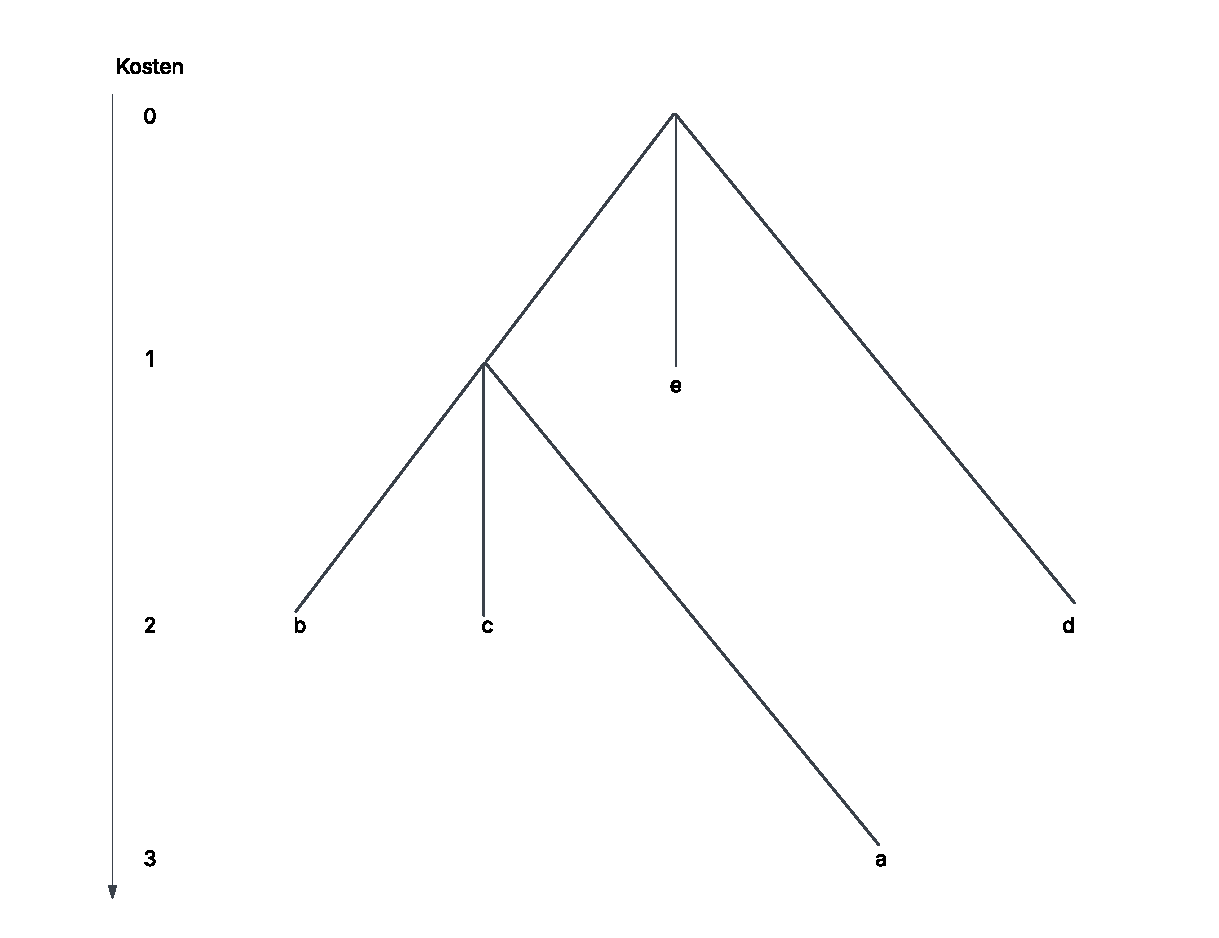
\includegraphics[width=0.6\textwidth]{Schmucknachrichten/pdf_src/lopsided_tree.pdf}
  \caption{lopsided tree: Perlendurchmesser: (1; 1; 2) }
  \label{fig:lopsided tree}
\end{figure}
Auch hier gilt: Jeder innerne Knoten muss mindestens zwei Kinder haben. Bei dieser Art von Bäumen hat jedoch nicht der rechteste Knoten die geringsten Kosten, sondern der oberste.
Die Kosten eines Knoten sind:
\begin{equation}
  K = K_E + K_S
\end{equation} 
wobei:\\
 - $K_E$ die Kosten seines Eltern Knoten sind\\
 - $K_S$ seine eigenen, neuen Kosten sind \\

 Der Algorithmus bleibt unverändert: Zunächst wird ein Baum erstellt, in dem alle Blätter ungefähr die gleichen Kosten haben. 
Anschließend wird der Buchstabe mit den höchsten Kosten nach oben verschoben, während der Baum unten erweitert wird.
Nach jedem Schritt werden die gesamt Kosten des Baums berechnet (Gleichung \eqref{equation:simple_kostenberechnung}) und mit den bisherigen besten verglichen. 
\\
Wenn die Druchmesser alle gleich groß sind, gilt: 
\begin{equation}
 p_i \cdot n_i = p_i \cdot \sum_n cp_n
\end{equation} 
daher kann der zweite Algorithmus sowohl für gleiche als auch unterschiedliche Durchmesser benutzt werden.


\clearpage
\section{Umsetzung}
Die Lösung wurde in Python3 geschrieben. Die Eingabetexte werden eingelesen. Die Durchmesser der Perlen werden in einer Liste gespeichert und der Text in einem string.
Aus dem Text werden anschließend zwei Listen erstellt: Die erste enthält die Häufigkeit der Buchstaben in absteigender Reihenfolge, die zweite listet die Buchstaben entsprechend dieser Sortierung auf.

\begin{figure}[h]
  \centering
  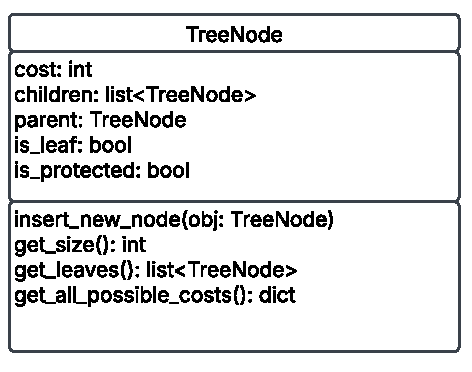
\includegraphics[width=0.6\textwidth]{Schmucknachrichten/pdf_src/klassen_diagramm.pdf}
  \caption{TreeNode Klasse}
  \label{fig:klassn_daigramm}
\end{figure}

\subsection{Erstellung des Baums}
Zu Beginn wird der Wurzelknoten, root, mit einem balancierten Baum.

\begin{lstlisting}[caption={Methode \texttt{create\_tree}}, label={lst:create_tree}]
  def create_tree(root: TreeNode) -> TreeNode:
\end{lstlisting}

Dabei werden jeweils alle potenziellen neuen Blätter im Baum betrachtet und das Blatt mit den geringsten Kosten wird dem Baum hinzugefügt.
Falls der Elternknoten ein Blatt ist, entsprechen die Kosten des neuen Blatts den kombinierten Kosten für die ersten beiden Blätter.
Das liegt daran, dass jeder innerne Knoten mindesten zwei Kinder haben muss – daher stellen diese Kosten die effektiv neu entstehenden Kosten für den Baum dar.
Das passiert solange, bis der der Baum genau soviele Blätter hat, wie es Buchstaben gibt.
Die möglichen neuen Blätter erhält man über den Aufruf
\begin{lstlisting}
  root.get_all_possible_costs()
\end{lstlisting}

\begin{lstlisting}[caption={Methode \texttt{get\_all\_possible\_costs}}, label={lst:get_all_pssible_costs}]
  def get_all_possible_costs(self) -> dict:
\end{lstlisting}
Die Methode prüft, ob das TreeNode-Objekt noch weitere Kinder aufnehmen kann und nicht protected ist.
Falls ja, fügt es sich selbst sowie die Kosten des potenziellen neuen Kindes einem Dictionary hinzu.
Anschließend wird die Methode rekursiv für alle bestehenden Kinder aufgerufen, sodass auch deren mögliche Erweiterungen im Dictionary erfasst werden.\\
\\
Neu Blätter werden über den Aufruf  
\begin{lstlisting}
  root.insert_new_node(obj)
\end{lstlisting} 
\vspace{-1.5em}
hinzugefügt
\vspace{2em} 
\begin{lstlisting}[caption={Methode \texttt{insert\_new\_node}}, label={lst:insert_new_node}]
  def insert_new_node(self, obj: TreeNode):
\end{lstlisting}
Die Methode prüft, ob das aktuelle Objekt selbst das gesuchte TreeNode Objekt ist. Falls ja, fügt es einen neues Kind hinzu. 
Wenn vorher noch keine Kinder vorhanden sind, werden zwei Kinder hinzugefügt.
Ansonsten wird die Methode rekursiv auf alle bestehenden Kinder angewandt.\\
\\
Über den Aufruf 
\begin{lstlisting}
  root.get_size()
\end{lstlisting} 
\vspace{-1.5em}
wird die Anzahl der Blätter ermittelt

\vspace{2em} 
\begin{lstlisting}[caption={Methode \texttt{get\_size}}, label={lst:get_size}]
  def get_size(self) -> int:
\end{lstlisting}
\vspace{0.5em}
Die Methode gibt 1 zurück falls das Objekt ein Blatt ist. Ansonsten wird die Methode rekursiv bei den Kinder aufgerufen und die Summe zurückgegeben

\subsection{Verbesserung des Baums}
Sobald ein balancierter Baum erstellt wurde, muss dieser optimiert werden. Dies geschieht über die Methode
\begin{lstlisting}[caption={Methode \texttt{find\_best\_tree}}, label={lst:find_best_tree}]
  def find_best_tree(root: TreeNode) -> TreeNode:
\end{lstlisting}


Die Methode versucht, den übergebenen Baum so lang zu optimieren, bis alle Blätter als $protected$ markiert sind.
Dazu wird der Optimierungsschritt wiederholt und jeweils die neuen Kosten des Baums berechnet.
Sind die neuen Kosten ein neues Minimum, wird der aktuelle Baum als bester Zwischenstand gespeichert.
Kann der Baum nicht weiter verbessern werden und es tritt ein Fehler auf, wird der bis dahin beste gefundene Baum zurückgegeben.\\
\\
Der Optimierungsschritt des Baums geschieht über die Methode
\begin{lstlisting}[caption={Methode \texttt{imporve\_tree}}, label={lst:imporve_tree}]
  def improve_tree(root: TreeNode) -> TreeNode:
\end{lstlisting}
Die Methode holt sich erstmal alle Blätter im Baum über den Aufruf
\begin{lstlisting}
  root.get_leaves()
\end{lstlisting}
\vspace{-1.5em}
Diese Liste wird dann aufsteigend sortiert und die Kosten für jedes Element können mit der Gleichung \eqref{Neue Kosten eines Buchstaben} berechnet werden.
Der Elternknoten des Blatts mit den höchsten Kosten wird daraufhin selbst zu einem Blatt. Dafür werden die Attribute vom Elternknoten
\begin{lstlisting}
  is_leaf = True
  is_protected = True
  children = []
\end{lstlisting}
\vspace{-1.5em}
gesetzt. Um die fehlenden Blätter wieder hinzuzufügen wird noch die Methde \ref{lst:create_tree} aufgerufen.\\
\\\\
Die gesamt Kosten des Baums wird durch die Methode 
\begin{lstlisting}[caption={Methode \texttt{calculate\_tree}}, label={lst:calculate_tree}]
  def calculate_tree(root: TreeNode) -> TreeNode:
\end{lstlisting}
berechnet. Die Methode holt sich erstmal alle Blätter im Baum über den Aufruf
\begin{lstlisting}
  root.get_leaves()
\end{lstlisting}
\vspace{-1.5em}
Die Liste wird dann aufsteigend sortiert und jedes Element wie in der Gleichung \eqref{Neue Kosten eines Buchstaben} berechnet und zusammenaddiert.





\clearpage
\section{Laufzeit und Diskussion}
\begin{figure}[h]
  \centering
  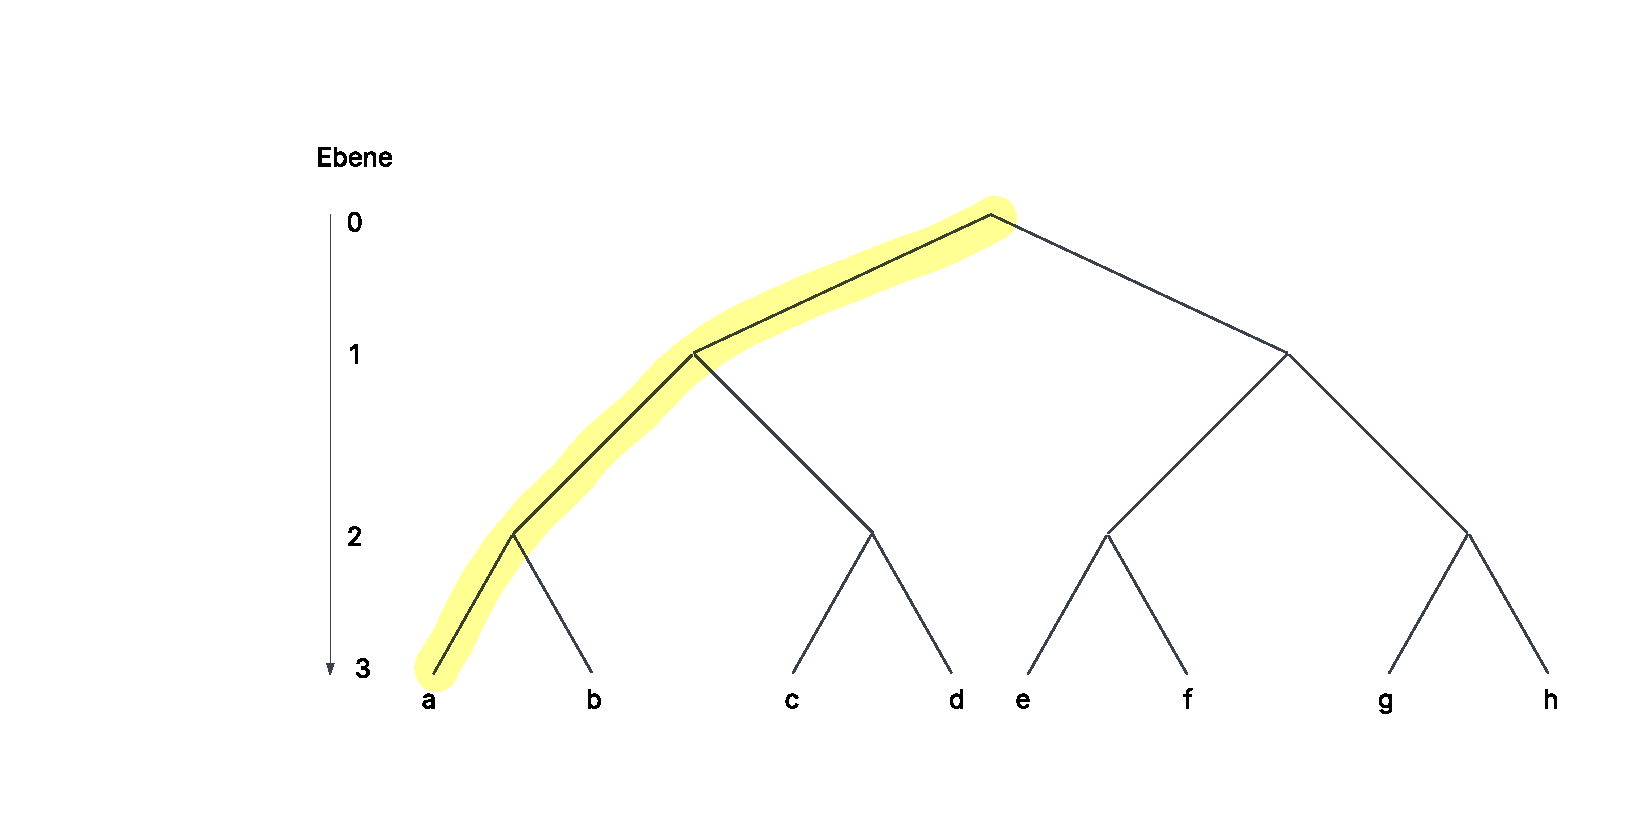
\includegraphics[width=0.6\textwidth]{Schmucknachrichten/pdf_src/trans_makiert.pdf}
  \caption{Balancierter Baum, richtige Knoten makiert}
  \label{fig:makiert_baum}
\end{figure}



\subsection{Analyse des Algorithmus}
Der Algorithmus endet, wenn keine Knoten mehr verschoben werden können.
Dies ist gegeben, wenn der Baum maximal links ausgeartet ist (Abbildung \ref{fig:baum_fertig}).
Allgemein kann jeder Knoten maximal $n-1$ Mal verschoben werden, bis er komplett auf der linken Seite ist. Dabei ist $n$ die Anzahl an verschieden Perlen.
Daraus folgt, dass es maximal 
\begin{equation}
  I < (n-1)\cdot\text{Anzahl falscher Knoten}
\end{equation}
Iteratioen benötigt werden, bis zum maximal ausgearteten Baum.
Falsche Knoten sind dabei innere Knoten, die beim ausbalancierten Baum noch nicht auf der richtigen Stelle sind, also alle bis auf die linkesten Knoten. (Abbildung \ref{fig:makiert_baum})

Generell gilt, um die maximale Anzahl an innere Knoten zu erhalten, sollte jeder Knoten eine möglichst wenig Kindern besitzen.
Wie zuvor festgelegt, hat jedere innere Knoten mindestens zwei Kinder. 
Daraus folgt, dass die maximale Anzahl an innere Knoten erreicht wird, wenn der Baum ein Binärbaum ist und kann durch
\begin{equation}
  \text{innere Knoten} = w - 1
\end{equation}
berchnet werden.
Dabei ist $w$ die Anzahl an Blättern/Codewörter.
Auf jeder Ebene existiert ein richtiger innere Knoten, derren Anzahl minimal mit 
\begin{equation}
  \text{richtige innere Knoten} = \log_{r-1}{w}
\end{equation}
abgeschäzt werden kann.\\
Daher ergibt sich
\begin{equation}
  I < (n-1)\cdot(w-1-\log_{r-1}{w})
\end{equation}
Dies bedeuted eine Laufzeit von $O(n\cdot w)$

\subsection{Stand der Forschung}
Die vorliegende Fragestellung ist seit den 60iger Jahren in der theorietischen Informatik bekannt. 
Dabei lieferte Huffman eine Lösung für den spezial Fall, von zwei Quellsymbolen.
\\
\\
Für unseren Fall von mehr als zwei Quellsymbolen mit unterschiedlichen Kosten, 
entwickelten Mordecai J. Golin und Günter Rote im Jahr 1998 das bis jetzt schnellste Verfahren, um auf eine exatke Lösung zu kommen.\\
"The minimum-cost prefix-free code for n words can be computed in $O(n^{C+2})$ time and $O(n^{C+1})$ space, if the costs of the letters are integers between 1 and C."\\
Für die Beispielaufgabe $schmuck5.txt$ hat der Algorithmus eine Laufzeit $34^8$(n=34; C=6) Iterationen. 
Dieser Art von Algorithmus kann wegen seiner Laufzeit nicht für die vorgegebenen Beispielaufgabe verwendet werden. [1]
\\
\\
Um eine polynominelle Laufzeit zu erreichen, entwickelten Mordecai J. Golin, Claire Mathieu und Neal E. Young 2012 ein approximations Verfahen.\\
Dieser Algorithmus passiert auf dem PTAS-Verfahren, wobei zuerst ein präfixfreier Code bis zur einer bestimmten Tiefe $\tau$ erstellt wird und dann die restlichen Codewörter durch ein Rundungsverfahren ergänzt werden.
Dabei ist es zentral, dass die Wahrscheinlichkeitsverteilung der zu kodierenden Codewörter möglichst in große Gruppen mit gleich großer Wahrscheinlichkeit ein geordnet werden können.
In den Beispielen, vorallem in Beispiel 9 ist dies nicht gegeben, weshalb das Bestimmen des Vorbaums über $9^{24}$ Schritte benötigt.
Somit ist dieses Verfahren für die gewählten Beispiele ebenfalls nicht verwendbar. [2]

\subsection{Fazit}
Der vorgestellte Algorithmus stellt keine exakte Lösung für das gegebene Problem dar, liefert jedoch in polynomieller Laufzeit eine gute Approximation.
Aus diesem Grund erfolgt durch das vorgestellte Verfahren keine Beantwortung, ob das Problem NP-hart ist.
Im Gegensatz zum oben vorgestellten Verfahren kann der Algorithmus auch Fälle verarbeiten, in denen die Wahrscheinlichkeiten der Zeichen nicht gleichmäßig verteilt oder in klaren Gruppen strukturiert sind.\\
In praktischen Tests zeigte sich, dass die berechneten Lösungen im Durchschnitt nur etwa 10\,\% von der optimalen Lösung abweichen.  
Ein formaler Beweis dieser Beobachtung steht allerdings noch aus.


\section{Beispiele}
Genügend Beispiele einbinden! Die Beispiele von der BwInf-Webseite sollten hier diskutiert werden, aber auch eigene Beispiele sind sehr gut – besonders wenn sie Spezialfälle abdecken. Aber bitte nicht 30 Seiten Programmausgabe hier einfügen!

\section{Quellcode}
Unwichtige Teile des Programms sollen hier nicht abgedruckt werden. Dieser Teil sollte nicht mehr als 2–3 Seiten umfassen, maximal 10.

\section{Quellen}

[1]  Mordecai J. Golin and Günther Rote,  \textit{A Dynamic Programming Algorithm for Constructing Optimal Prefix-Free Codes with Unequal Letter Costs}, IEEE Transactions on Information Theory 44, no. 5, (September 1998)

[2] Mordecai J. Golin, Claire Mathieu und Neal E. Young, \textit{HUFFMAN CODING WITH LETTER COSTS: A LINEAR-TIME APPROXIMATION SCHEME}, 2012 Society for Industrial and Applied Mathematics
Vol. 41, No. 3, pp. 684–713



\end{document}
